\section{pytorch.autograd}

\subsection{autograd表层机制}
\begin{itemize}
\item
  主要参照了这篇文章的内容\href{https://towardsdatascience.com/getting-started-with-pytorch-part-1-understanding-how-automatic-differentiation-works-5008282073ec}{Getting
  Started with PyTorch Part 1: Understanding how Automatic
  Differentiation works}
\item
  文章中提到的Variables在官方文档\href{https://pytorch.org/docs/stable/autograd.html\#variable-deprecated}{Variable
  (deprecated)}里面说到已经被deprecated了。因为Tensor已经支持requires\_grad=True,所以Variables不再使用,将其当成Tensor即可。
\item
  torch 的 autograd机制如下:

  \begin{itemize}
  \tightlist
  \item
    autograd使用的是动态计算图机制
  \item
    动态计算图主要是从输入到输出的一个计算图,以中间的计算作为节点
  \item
    比如文章里面提到的,下面一个计算图,a为一个Tensor(输入,也为叶子节点),L为结果(输出,也为root)
  \end{itemize}

\begin{verbatim}
b = w1 * a
c = w2 * a
d = (w3 * b) + (w4 * c)
L = 10 - d
\end{verbatim}

  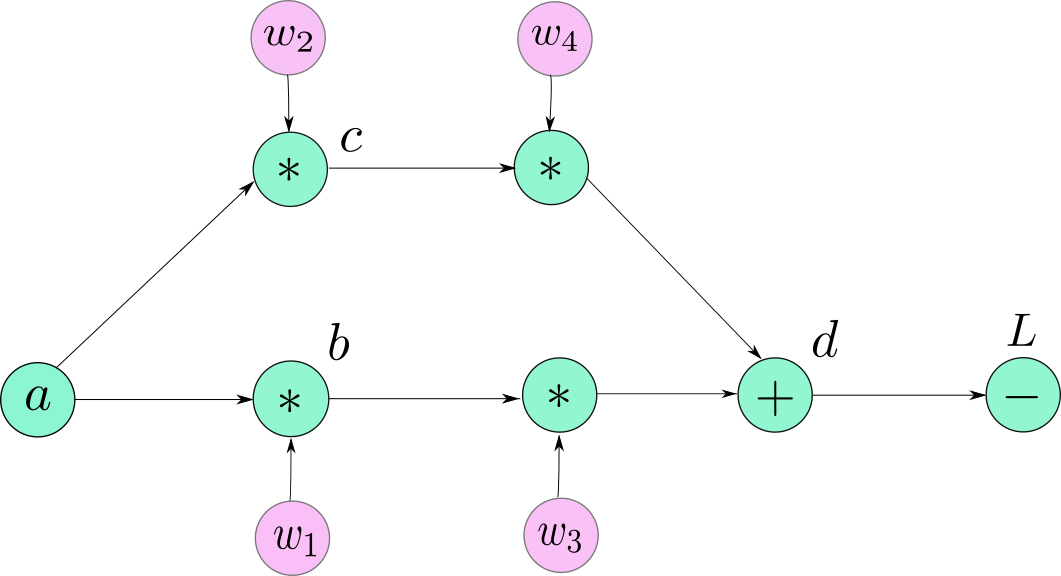
\includegraphics[width=0.8\linewidth]{pytorch/pic/4-9.png}

  \begin{itemize}
  \tightlist
  \item
    计算图是动态创建的,也即运算时才会动态的创建出来
  \item
    叶子节点也只有在对其进行运算时才会产生计算图
  \item
    计算节点可以自己定义,在官方文档\href{https://pytorch.org/docs/stable/notes/extending.html}{Extending
    PyTorch}提到了怎样定义自己的计算
  \item
    计算图在反向传播时只会对requires\_grad=True的节点计算梯度
  \item
    由于Tensor对Tensor求导会导致奇怪的事情,所以在需要这个的时候需要提供对应的系数向量Tensor。比如Tensor
    y 想要求微分,需要使用 torch.autograd.backward(y,
    w),w是和y相同类型的Tensor。torch实际上是先计算 l = torch.sum(y *
    w),然后求 l 对(能够影响到 y 的)所有变量 x
    的导数。这里的解释来自于文章\href{https://zhuanlan.zhihu.com/p/29923090}{PyTorch
    的 backward 为什么有一个 grad\_variables 参数?}。
  \end{itemize}
\end{itemize}

\subsubsection{计算图的一些特点}

\begin{itemize}
\tightlist
\item
  计算图的节点是复用的,也即下面代码中,m的计算图和n的计算图都包含相同的计算节点y。所以m
  backward之后,n就不能再backward了,因为y的buffer已经被freed了。
\item
  计算图中的梯度计算是累加的,也即上一次的梯度如果没清除的话,下一次再次计算梯度时会加上上一次的梯度。清除x的梯度可以使用
  x.grad.data.zero()
\item
  想要让计算图保留中间的buffer,可以在backward时加上参数retain\_graph=True
\item
  计算图只会保留叶子节点(即普通创建的Tensor,没有其他计算操作,如下面的变量x)的梯度,中间节点的梯度不会保留(如下面的y)。想要保留的话,如y,使用
  y.retain\_graph()
\end{itemize}

\begin{lstlisting}
import torch

x = torch.randn(2, 2, requires_grad=True)
y = 2 * x
m = y.mean()
n = y.sum()

m.backward()
print(y.grad)       # should be empty, because y is not leaf node
n.backward()    # should be error here, because y's buffer freed before

x.grad.data.zero_()    # clear x.grad
y = x ** 2
m = y.mean()
n = y.sum()
m.backward(retain_graph=True)
n.backward()    # should work now, because y's buffer still there

x.grad.data.zero_()    # clear x.grad
y = x * 3
y.retain_graph()
m = y.mean()
m.backward()
print(y.grad)	# can see y's grad now
\end{lstlisting}

\subsubsection{遇到的问题}

\begin{itemize}
\tightlist
\item
  在尝试torch的自动微分时,遇到一个奇怪的问题。上面说了一个计算图只能backward一次,backward多次会报错。然而如果在计算中只用到了加号和减号,那么可以backward多次,且每一次backward会使得微分值不断增长,比如一次正常微分x的微分值为0.5,那么两次微分值为1,3次微分值为1.5。具体可见下面代码。
\end{itemize}

\begin{lstlisting}
import torch
x = torch.randn(2, 2, requires_grad=True)
y = x + x - x + 3
z = y.mean()
z.backward()
print(x.grad)    # will be tensor([[0.2500, 0.2500], [0.2500, 0.2500]])
z.backward()	# no error here
print(x.grad)	# will be tensor([[0.5000, 0.5000], [0.5000, 0.5000]])
# you can continue backward if you like
\end{lstlisting}

\begin{itemize}
\tightlist
\item
  查了一下,在stackoverflow中,有人回答了\href{https://stackoverflow.com/questions/52463439/pytorch-can-backward-twice-without-setting-retain-graph-true}{这个问题}。这个是由于计算过于简单导致没有中间的buffer产生,所以backward的时候不会有buffer被freed掉,因此可以多次backward。
\end{itemize}

\subsection{autograd具体实现}

\begin{itemize}
\tightlist
\item
  源码见:https://github.com/pytorch/pytorch/
\item
  在文件
  \href{https://github.com/pytorch/pytorch/blob/master/torch/autograd/__init__.py\#L38}{torch/autograd/\_\_init\_\_.py
  的backward方法},最后调用了Variable.\_execution\_engine.run\_backward
\item
  在文件
  \href{https://github.com/pytorch/pytorch/blob/master/torch/autograd/variable.py}{torch/autograd/variable.py}
  中,\_execution\_engine使用的是torch.\_C模块里面的\_ImperativeEngine
\item
  调查发现torch.\_C是使用c++编写的模块, c++ 源码在
  \href{https://github.com/pytorch/pytorch/tree/master/torch/csrc}{torch/csrc}目录下
\item
  python使用c++接口见:https://docs.python.org/3.7/extending/extending.html
\end{itemize}

\subsubsection{torch.\_C模块}

\begin{itemize}
\item
  setup.cpp L633里面extensions 包含了torch.\_C模块的编译,编译的源文件是
  \href{https://github.com/pytorch/pytorch/blob/master/torch/csrc/stub.cpp}{torch/csrc/stub.cpp}
\item
  \href{https://github.com/pytorch/pytorch/blob/master/torch/csrc/stub.cpp}{torch/csrc/stub.cpp}
  包含了头文件Python.h,定义了如何初始化模块
  \texttt{\_C},实际上使用的是
  \href{https://github.com/pytorch/pytorch/blob/master/torch/csrc/Module.cpp\#L542}{torch/csrc/Module.cpp
  中的 \texttt{initModule}} 函数

  \begin{itemize}
  \tightlist
  \item
    \texttt{initModule} 函数给 torch.\_C
    添加了一系列的模块方法,autograd、cuda、Variable、Function、Engine的方法也在其中
  \end{itemize}
\item
  \texttt{\_ImperativeEngine}:在
  \href{https://github.com/pytorch/pytorch/blob/master/torch/csrc/Module.cpp\#L587}{torch/csrc/Module.cpp
  L587} 添加了引擎
  \texttt{THPEngine},其就是在autograd中使用的\texttt{\_ImperativeEngine},详见文件
  \href{https://github.com/pytorch/pytorch/blob/master/torch/csrc/autograd/python_engine.cpp}{torch/csrc/autograd/python\_engine.cpp}
  中的THPEngine\_initModule方法。

  \begin{itemize}
  \tightlist
  \item
    这个\texttt{\_ImperativeEngine}定义为:\texttt{PyTypeObject\ THPEngineType},详见
    torch/csrc/autograd/python\_engine.cpp
    \href{https://github.com/pytorch/pytorch/blob/master/torch/csrc/autograd/python_engine.cpp\#L227}{L227}
  \item
    里面有方法\texttt{run\_backward}
  \end{itemize}

\begin{lstlisting}
static struct PyMethodDef THPEngine_methods[] = {
  {(char*)"run_backward", (PyCFunction)THPEngine_run_backward, METH_VARARGS | METH_KEYWORDS, nullptr},
  {(char*)"queue_callback", (PyCFunction)THPEngine_queue_callback, METH_O, nullptr},
  {(char*)"is_checkpoint_valid", (PyCFunction)THPEngine_is_checkpoint_valid, METH_NOARGS, nullptr},
  {nullptr}
};
\end{lstlisting}


  \begin{itemize}
  \tightlist
  \item
    run\_backward里面检查并处理参数后,在
    \href{https://github.com/pytorch/pytorch/blob/master/torch/csrc/autograd/python_engine.cpp\#L169}{L169}
    调用\texttt{engine.execute},这个是\texttt{PythonEngine::execute},其又调用了
    \texttt{Engine::execute}
  \end{itemize}
\end{itemize}

\hypertarget{engineexecute}{%
\subsubsection{Engine::execute()}\label{engineexecute}}

\begin{itemize}
\tightlist
\item
  在文件
  \href{https://github.com/pytorch/pytorch/blob/master/torch/csrc/autograd/engine.cpp\#L562}{torch/csrc/autograd/engine.cpp
  L562},其在一开始调用\texttt{std::call\_once(start\_threads\_flag,\ \&Engine::start\_threads,\ this);}

  \begin{itemize}
  \tightlist
  \item
    \texttt{start\_threads}创建多个线程,并为每个线程创建一个任务队列\texttt{ready\_queue}

    \begin{itemize}
    \tightlist
    \item
      线程创建:\texttt{std::thread\ t(\&Engine::thread\_init,\ this,\ i\ -\ 1);},\texttt{thread\_init}又调用了\texttt{thread\_main}
    \item
      \texttt{thread\_main}里面等待分配任务,分配任务task后,调用\texttt{evaluate\_function(task);},里面又调用\texttt{call\_function(task)}
    \item
      \texttt{call\_function}里面调用task里面的 \texttt{fn}
      (\texttt{Function}),也即每个Variable的\texttt{gradient\_edge}

      \begin{itemize}
      \tightlist
      \item
        \texttt{gradient\_edge}如果是叶子节点(需要求grad的Tensor),其为\texttt{accumulator}累加器,不是叶子节点为\texttt{grad\_fn}
      \item
        \texttt{Function}的\texttt{operate()}会调用不同Function的\texttt{apply}方法,即不同的Function会重载\texttt{apply}方法
      \end{itemize}
    \item
      调用\texttt{fn}的参数来自于函数\texttt{call\_pre\_hooks},到这里卡住了,\texttt{call\_pre\_hooks}里需要的\texttt{FunctionPreHook}是个虚基类,应该在具体的\texttt{Function}实现中会实现这个类
    \end{itemize}
  \end{itemize}
\end{itemize}

\hypertarget{autogradux5177ux4f53ux5b9eux73b0ux5927ux81f4ux7b97ux6cd5}{%
\subsubsection{autograd具体实现大致算法}\label{autogradux5177ux4f53ux5b9eux73b0ux5927ux81f4ux7b97ux6cd5}}

\begin{lstlisting}
b = a * a
c = b + a
out = b + c
\end{lstlisting}

\begin{enumerate}
\def\labelenumi{\arabic{enumi}.}
\tightlist
\item
  为每个设备分配一个优先级队列,并创建对应数量的thread(一个thread是CPU,其他thread是GPU),\href{https://github.com/pytorch/pytorch/blob/master/torch/csrc/autograd/engine.cpp\#L682}{torch/csrc/autograd/engine.cpp
  L682}

  \begin{itemize}
  \tightlist
  \item
    thread的具体执行函数为\texttt{thread\_main},位于\href{https://github.com/pytorch/pytorch/blob/master/torch/csrc/autograd/engine.cpp\#L268}{torch/csrc/autograd/engine.cpp
    L268}
  \item
    这个函数以设备号从\texttt{ready\_queues}(type:
    哈希表)中取出对应的优先级队列,block直到队列里面有任务
  \item
    优先队列的优先级为开始执行时间短的任务优先(空的任务更优先,暂时不知道为什么有空任务),见\href{https://github.com/pytorch/pytorch/blob/master/torch/csrc/autograd/engine.cpp\#L70}{torch/csrc/autograd/engine.cpp
    L69}
  \item
    执行任务的具体函数为\texttt{evaluate\_function},见\href{https://github.com/pytorch/pytorch/blob/master/torch/csrc/autograd/engine.cpp\#L437}{torch/csrc/autograd/engine.cpp
    L436}
  \end{itemize}
\item
  对根节点(即backward开始的节点的grad\_fn),统计dependencies

  \begin{itemize}
  \tightlist
  \item
    对应于\href{https://github.com/pytorch/pytorch/blob/master/torch/csrc/autograd/engine.cpp\#L582}{torch/csrc/autograd/engine.cpp
    L582},\texttt{compute\_dependencies(graph\_root.get(),\ graph\_task);},具体实现:\href{https://github.com/pytorch/pytorch/blob/master/torch/csrc/autograd/engine.cpp\#L526}{torch/csrc/autograd/engine.cpp
    L526}
  \item
    这个dependencies就是节点grad\_fn的依赖关系,比如上面的代码中正在计算out的\texttt{+}的backward,那么把b的\texttt{*}和c的\texttt{+}加入dependencies,其中b的\texttt{*}的dependencies值是2,c是1
  \item
    这个依赖关系指只有相应的计算节点所需的上层的依赖的grad都计算完才能继续计算这个节点,比如out的\texttt{+}的grad计算完,计算c的\texttt{+}
  \item
    这个依赖目前我认为应该是为了让b的\texttt{*}只计算一次
  \end{itemize}
\item
  将根节点grad\_fn加入优先队列,开始计算grad,见\href{https://github.com/pytorch/pytorch/blob/master/torch/csrc/autograd/engine.cpp\#L586}{torch/csrc/autograd/engine.cpp
  L585},\texttt{ready\_queue(at::kCPU).push(FunctionTask(\&graph\_task,\ std::move(graph\_root),\ InputBuffer(0)));}
\item
  当一个grad\_fn节点计算完,会有一个outputs,对应于依赖的每个grad\_fn的grad,比如上面out的\texttt{+}就会生成b的\texttt{*}和c的\texttt{+}
  两个grad,如果当前依赖为0,那么把对应的grad\_fn节点加入相应设备的优先队列,比如此时c的\texttt{+}

  \begin{itemize}
  \tightlist
  \item
    这个output的grad放入对应节点的inputBuffer里面,然后传入节点的多个grad会加起来,\texttt{input\_buffer.add(next.input\_nr,\ std::move(output));},具体实现:\href{https://github.com/pytorch/pytorch/blob/master/torch/csrc/autograd/input_buffer.cpp\#L15}{torch/csrc/autograd/input\_buffer.cpp
    L15}
  \item
    具体细节见\texttt{evaluate\_function}函数,\href{https://github.com/pytorch/pytorch/blob/master/torch/csrc/autograd/engine.cpp\#L475}{torch/csrc/autograd/engine.cpp
    L475}
  \end{itemize}
\end{enumerate}

\subsubsection{pytorch 模块结构}

\begin{itemize}
\tightlist
\item
  aten文件夹:Tensor底层的实现
\item
  torch文件夹:Tensor较为高层的实现
\item
  c10文件夹:后面社区会把aten迁移到这里面,目前里面已经有Tensor的内存管理`
\item
  具体参考文章:\href{https://oldpan.me/archives/pytorch-build-simple-instruction}{Pytorch源码编译简明指南}和\href{https://zhuanlan.zhihu.com/p/55204134}{PyTorch的编译系统}
\end{itemize}
